
\section*{Общая характеристика работы}

\newcommand{\actuality}{\underline{\textbf{\actualityTXT}}}
\newcommand{\progress}{\underline{\textbf{\progressTXT}}}
\newcommand{\aim}{\underline{{\textbf\aimTXT}}}
\newcommand{\tasks}{\underline{\textbf{\tasksTXT}}}
\newcommand{\novelty}{\underline{\textbf{\noveltyTXT}}}
\newcommand{\influence}{\underline{\textbf{\influenceTXT}}}
\newcommand{\methods}{\underline{\textbf{\methodsTXT}}}
\newcommand{\defpositions}{\underline{\textbf{\defpositionsTXT}}}
\newcommand{\reliability}{\underline{\textbf{\reliabilityTXT}}}
\newcommand{\probation}{\underline{\textbf{\probationTXT}}}
\newcommand{\contribution}{\underline{\textbf{\contributionTXT}}}
\newcommand{\publications}{\underline{\textbf{\publicationsTXT}}}
\newcommand{\workrequirements}{\underline{\textbf{\workrequirementsTXT}}}


{\actuality} Обзор, введение в тему

{\aim} данной работы является \ldots


{\novelty}
\begin{enumerate}
  \item Впервые \ldots
  \item Впервые \ldots
  \item Было выполнено оригинальное исследование \ldots
\end{enumerate}

{\influence} \ldots

{\methods} \ldots

{\probation} \ldots

{\contribution} Автор принимал активное участие \ldots

 % Характеристика работы по структуре во введении и в автореферате не отличается (ГОСТ Р 7.0.11, пункты 5.3.1 и 9.2.1), потому её загружаем из одного и того же внешнего файла, предварительно задав форму выделения некоторым параметрам

%Диссертационная работа была выполнена при поддержке грантов ...

\underline{\textbf{Объем и структура работы.}} Диссертация состоит из введения, четырёх глав, заключения и двух приложений. Полный объём диссертации составляет 175 страницу с 13 рисунками и 12 таблицами. Список литературы содержит 96 наименований.

%\newpage
\section*{Содержание работы}
Во \underline{\textbf{введении}} обосновывается актуальность
исследований, проводимых в~рамках данной диссертационной работы,
приводится обзор научной литературы по изучаемой проблеме,
формулируется цель, ставятся задачи работы, излагается научная новизна
и практическая значимость представляемой работы. В~последующих главах
сначала описывается общий принцип, позволяющий ..., а~потом идёт
апробация на частных примерах: ...  и~... .

% SYNOPSIS_1 >>> related_work.tex
\underline{В \textbf{первой главе}} рассматриваются известные подходы к решению задач в направлении выявления семантической информации, проводится их анализ, выявляются недостатки. После чего автором описывается использованная в настоящей диссертации методология. Эта методология призвана решить недостатки в существующих моделях определения смысловой близости объектов информационных систем по их ключевым словам.

В первом разделе проводится библиографический обзор существующих методов, выделяются сильные и слабые стороны моделей. Анализу подвергаются работы, в которых исследуются семантическая близость для пар слов и пар коротких предложений естественного языка. В частности, обозреваются работы, связанные с анализом ключевых слов.

Второй раздел содержит в себе выводы из обзора и указывает на недостатки рассмотренных методов и на причины неприменимости этих методов к решаемым в данной работе задачам.

В заключающем разделе главы вводится методология, используемая автором в последующих главах для разработки моделей семантической близости. Показывается целесообразность и необходимость рассмотренной методологии, ее преимущества в сравнении с уже существующими. Стоит также отметить, что отдельные пункты методологии представляют собой самостоятельный интерес.
% related_work.tex <<< SYNOPSIS_1


% SYNOPSIS_2 >>> word_similarity.tex
\underline{Во \textbf{второй главе}} подробно описываются разработанные автором эвристические модели, алгоритмы и реализующее их программное обеспечение для определения семантической близости пары ключевых слов. Разработанные автором на основе проведенных исследований с использованием полученных в их ходе эвристических соображений модели определения семантической близости, являются важным результатом деятельности в рамках подготовки настоящей диссертации.

Задача, решение которое представлено в данной главе, имеет следующую математическую постановку. Дано множество объектов системы $D$ и множество ключевых слов $W$. Каждый элемент $d_i \in D$ представлен \emph{набором ключевых слов} $t_i \in T$, состоящим из  $k_i$ ключевых слов из множества $W$:

$$d_i\rightarrow t_i = (w_{i_1},w_{i_2},...,w_{i_{k_i}}).$$

Здесь $T$ - множество всех наборов ключевых слов или \emph{коллекция ключевых слов}. Множество $T$ состоит из \emph{уникальных наборов ключевых слов}. Наборы ключевых слов совпадают, если существует перестановка, отождествляющая эту пару наборов. Кроме того, между объектами системы заданы отношения различных типов, определенные направленным графом $G_{rel} = (D, R)$, в котором $D$ - множество вершин (объекты системы), а $R$ - ребра, определяющие отношения. Ребра этого графа помечены типом отношения: $l: R \rightarrow T$, где $T$ - множество возможных типов.  Множества $(D, T, W, G_{rel})$ задают модель информационной аналитической системы.

В рамках данной главы необходимо разработать модель определения семантической близости и в ее рамках такую функцию близости $f : W \times W \rightarrow [0, 1]$, б\'ольшие значения которой означали бы сильный уровень смысловой близости между ключевыми словами.

Для определения близости вводятся вспомогательные графы, вершинами которых являются ключевые слова, а ребра указывают на некоторые свойства пары ключевых слов. В самом простом виде таким свойством может являться факт причастности пары ключевых слов одному набору. Кроме этого существуют более сложные и неявные связи между парами ключевых слов. Примером такой связи служить \emph{контекстная близость}, определенная в главе \ref{cont_sim}. Согласно введенной модели, такая близость устанавливается между парой ключевых слов $w_a$ и $w_b$ в том случае, если существует большое число ключевых слов, которые входят одновременно и в наборы, содержащие слово $w_a$, и в наборы, содержащие слово $w_b$. Это означает, что если для пары слов существует достаточное количество общих <<соседей по набору>>, то между ними проявляется такая контекстная связь.
% word_similarity.tex <<< SYNOPSIS_2

% SYNOPSIS_2.1 >>>
В разделе 2.1 описывается модель близости, названная \emph{WordContSim}. Начало раздела посвящается введению вспомогательного графа ключевых слов, после чего приводится описание и аргументация эвристических идей, заложенных в данную модель. Следующим этапом изложения является представление реализающих данную модель алгоритмов, асимптотических оценок вычислительной сложности и затрат по памяти для их программных реализаций.
% <<< SYNOPSIS_2.1

% SYNOPSIS_2.2 >>>
Раздел 2.2 посвящен понятию степени абстрактности (далее для краткости - абстрактности) ключевого слова. Под абстрактностью ключевого слова понимается степень общности значения этого слова. Абстрактность будет использована в дальнейшем для решения задачи определения тематики набора ключевых слов, поставленной в разделе \ref{theme_tags}. Кроме того, она нашла применение в модели семантической близости пары ключевых слов, описанной в разделе \ref{ml_sim}.

Задача, решаемая автором в настоящем разделе, формулируется следующим образом. Рассматривается модель аналитико-информационной системы, введенная в начале настоящей главы. Необходимо по коллекции ключевых слов $T$ и множества $W$ ключевых слов данной коллекции разработать такую меру абстрактности
    $$a_T : W \rightarrow \mathbb{R}+,$$
%
чтобы б\`ольшим значениям меры соответствовали слова более широкого значения, а меньшим - слова более конкретного, обладающего определённой спецификой значения.

В настоящем разделе представлены алгоритмы определения степени абстрактности ключевых слов на основе графа ключевых слов, введенного в начале данной главы. В наборах ключевых слов $t \in T$ коллекции $T$ присутствуют слова, которые
указывают на общую тематическую направленность документа, а также слова, отражающие более узкую специализацию (термины). Проиллюстрируем это на примере наукометрической системы и следующих наборов ключевых слов, ассоциированных с научными публикациями (подчёркнуты слова более общего значения):

    \textbf{[рынок труда, профессиональная ориентация, \underline{прогнозирование}, \underline{модель}, \underline{алгоритм}]}\

    \textbf{[внеаудиторная работа, учебный проект, целеустремленность, \underline{творчество}]}\

    \textbf{[компетентностный подход, система компетенций, межпредметная интеграция, \underline{моделирование}, \underline{математика}, \underline{естественно-научные дисциплины}]}\

По ключевым словам, выделенным в каждом из наборов, трудной процедурой является понять специфику научной работы, соответствующей этим ключевым словам. Такие слова, как \emph{математика, естественно-научные дисциплины} могут определить тематическую направленность документа, но конкретику добавляют остальные слова (не подчеркнутые слова наборов). В рамках поставленной задачи необходимо уметь отличать слова более общего значения от узкоспециальных по смыслу слов. 
    
Важным в практическом плане является решение задачи, напрямую вытекающей из задачи определения уровня абстрактности. Эта задача состоит в том, чтобы по коллекции наборов ключевых слов системы научиться определять \emph{тематические ключевые слова}. Тематические ключевые слова - такие ключевые слова аналитической системы, которые определяют тематическую направленность или предметную область документа системы. Далее приводится пример, иллюстрирующий данное определение.

Для наукометрической системы тематическими ключевыми словами могут являться, например, названия дисциплин: \emph{вычислительная математика, теория чисел, теория вероятности}. С одной стороны эти слова не являются слишком абстрактными и представляется возможным определить предметную область документа по ним. С другой стороны, смысл этих слов не слишком специфичен. Эти слова понятны любому пользователю системы, а не только узкопрофильному специалисту.

Таким образом, можно разбить все множество ключевых слов $W$ на перечисленные далее три уровня в зависимости от степени абстрактности этих слов.
\begin{itemize}
    \item \textbf{Термины}. Наиболее узкоспециальные по смыслу ключевые слова. Примерами терминов являются: \emph{цитовир-3, титаносиликаты, двухфазные струи}.
    \item \textbf{Тематические ключевые слова}. Ключевые слова, определяющие тематическую направленность документа. Примерами таких слов являются: \emph{психология,физика, педагогическая деятельность}.
    \item \textbf{Абстрактные ключевые слова}. Слова, наиболее абстрактные по смыслу. Примеры абстрактных слов - \emph{задача, моделирование, концепт, система, технология, методология}.
\end{itemize}

Умение определять тематические ключевые слова полезно в том числе и тем, что позволяет строить автоматические классификаторы и рубрикаторы для заданной системы.
% <<< SYNOPSIS_2.2

% >>> SYNOPSIS_2.3
В главе 2.3 рассматриваются методы улучшения качества определения семантической близости для пары ключевых слов с помощью методов машинного обучения с учителем. В тексте подробно описывается сведение рассматриваемой задачи к задаче классификации, то есть к задаче определения целевой метки заданного объекта из заранее сформированного множества меток. Обучение с учителем подразумевают использование обучающей выборки - множества объектов, для которой известны истинные целевые метки. Эта выборка необходима для тренировки модели машинного обучения. Обученная модель машинного обучения применяется к произвольному объекту системы и выдает предсказанную целевую метку.

Сбор обучающего набора данных является обычно трудоемкой и дорогой работой: как правило для процесса требуется как минимум несколько экспертов в направлении, для которого собираются тренировочное множество. Более того, для некоторых задач, в число которых входит и задача определения семантической близости пар ключевых слов, является сложным даже правильно составить инструкцию для экспертов для правильной оценки примеров. Это происходит по причине того, что семантическая близость - субъективная величина и сильно зависит от области применения, контекста, человека и задачи. Например, слово <<стол>> может быть близким по смыслу для слова <<стул>> из бытовых соображений. В то же время если бы эти два слова были синонимами (а следовательно взаимозаменяемыми) в информационной системе, представляющей интернет-магазин, продающий мебель, то имела бы место ситуация, когда пользователь ищет один из этих предметов, а в поисковой выдаче получает другой, что является недопустимым. Рассмотренные в следующих далее разделах алгоритмы сбора обучающего множества призваны разрешить обозначенные проблемы.

Автором настоящей диссертации были разработаны два метода получения обучающих примеров без задействия в процесс экспертов. Первый из них включает в себя набор эвристических алгоритмов создания обучающей выборки. Второй является полностью автоматическим методом и строится исключительно при помощи описанных в предыдущих главах графовых моделей представления данных. Важнейшим преимуществом этого метода является его универсальность и применимость не только к задачам определения семантической близости, но и к любым другим задачам, в которых объекты системы представляются в виде некоторого графа и имеется необходимость в классификации отношений между парой объектов. Также универсальность проявляется в том, что выборка строится непосредственно по данным и не использует никакие внешние источники. Это позволяет определить отношение близости специфичные для конкретной системы. Другое преимущество метода в возможности использовать эффективные модели машинного обучения с учителем, вместо более слабых моделей без учителя, которые, к тому же представляется сложным валидировать без обучающих примеров.
% SYNOPSIS_2.3 <<<

% >>> SYNOPSIS_2.4
В разделе 2.4 описывается построение тезауруса ключевых слов по коллекции наборов ключевых слов. Схема построения построения приводится на рисунке \ref{img:thes}.

\begin{figure}[ht]
  \begin{minipage}[ht]{1.0\linewidth}\centering
    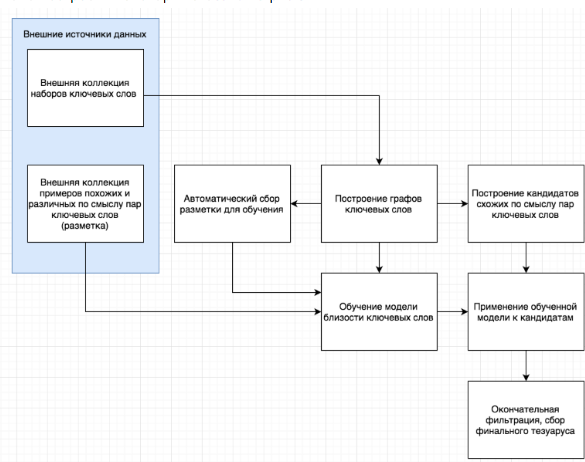
\includegraphics[width=0.7\linewidth]{Dissertation/pics/thes}
    \caption{Схема построения словаря тезауруса ключевых слов}
  \end{minipage}
  \label{img:thes}
\end{figure}

В качестве внешних данных используется коллекция наборов ключевых слов научных публикаций, собранная из сети Веб. Это коллекция, насчитывающая сотни тысяч наборов ключевых слов для русскоязычных статей и миллиона наборов на английском языке. С помощью этих наборов поочередно строится несколько графов близости. Одним из таких графов является, например, граф, в вершинах которого находятся ключевые слова, а в ребро означает причастность двух ключевых слов одному набору. Вес ребра тем больше, чем чаще пара слов встречается в одном наборе. Другим примером контекстного семантического графа является граф, в вершинах которого как и прежде стоят ключевые слова, а ребра указывают на наличие у этой пары общего ключевого слова, которое входит в некоторые наборы вместе и с первым словом из пары, и со вторым (но не с двумя сразу). Было показано, что ребра такого графа гораздо сильнее отражают семантическую близость, в то время как ребра первого графа служат для улучшения механизмов поисковых подсказок, потому что предлагают связанные, но более разнообразные слова для заданного.

% SYNOPSIS_2.4 <<<

% SYNOPSIS_2.5 >>> сам написал, в диссере нет
В заключительном разделе главы приводятся преимущества и недостатки разработанных решений в направлении исследования моделей семантической близости пары ключевых слов.
% <<< SYNOPSIS_2.5 

% SYNOPSIS_3 >>>
В \underline{\textbf{третье главе}} представлены разработанные автором настоящей работы алгоритмы выявления смысловой близости между двумя наборами ключевых слов.  Этот уровень определяет уровень близости пары объектов интеллектуальной системы, с которыми были ассоциированы данные наборы ключевых слов.
Семантическая близость между наборами ключевых слов определяется с использованием введенной  в предыдущей главе методах определения семантической близости между парой ключевых слов.
% <<< SYNOPSIS_3

% >>> SYNOPSIS_3.1

В разделе 3.1 описываются модели и алгоритмы определения смысловой близости наборов ключевых слов. 

Решаемая задача имеет следующую постановку. Дано множество документов $D$ и множество ключевых слов $W$. Каждый элемент $d_i \in D$ представлен набором из $k_i$ ключевых слов из множества $W: d_i = (w_{i,1},w_{i,2},...,w_{i,ki})$. Необходимо разработать такую функцию близости $TupleSim : 2^W \times 2^W \rightarrow [0, 1]$, высокие значения которой означали бы высокий уровень смысловой близости между наборами и, следовательно, соответствующими документами системы. 

Также к разрабатываемой метрике предъявляются следующие требования:
\begin{itemize}
    \item программная реализация должна быть способна вычислять значения метрики в режиме реального времени. Значительные задержки между отправленным пользователем запросом и полученным ответом не могут быть слишком долгими, иначе использование такой системы будет трудновыполнимым;
    \item необходимо уметь посчитать близость в том числе и для тех наборов, слова которых не представлены в системе. Существенная доля поисковых запросов содержит слова, которые ранее не были заданы ни разу и, что более важно, не встречаются в описаниях к документам системы.
\end{itemize}

Основой для разрабатываемой функции определения близости являются методы и средства, введенные в предыдущей главе. Таким образом, в качестве базовых  блоков определения близости наборов естественно положить идеи о близости между словами, из которых эти наборы состоят. Формально это можно описать как $TupleSim(d_i, d_j) = TupleSim(WordSim(w_{i,1}, w_{j,1}), ... , WordSim(w_{i,ki}, w_{j,kj}))$. 

% SYNOPSIS_3.1 <<<

% >>> SYNOPSIS_3.2

В разделе 3.2 описывается решение задачи определения тематической направленности набора ключевых слов и дается разработанное автором настоящей диссертации решение.

Пусть, как и ранее, дано множество документов $D$ и множество ключевых слов $W$. Каждый элемент $d_i \in D$ представлен набором из $k_i$ ключевых слов из множества $W: di = (w_{i,1},w_{i,2},...,w_{i,ki})$. Необходимо разработать методы определения тематики для каждого документа коллекции. Под тематикой следует понимать название некоторой области знаний, дисциплины, специальности или направления. Определив такое слово для документа, можно с высокой вероятностью сказать о чем этот документ. Тематическое ключевое слово - это такое ключевое слово из $W$, которое может являться тематикой документа. Таким образом, необходимо из множества ключевых слов $W$ выделить подмножество $T \subset W$ тематических ключевых слов и для каждого документа из коллекции определить соответствующее ему множество тематических ключевых слов, т.е. определить отображение $t : D \rightarrow 2^T$ . Отметим, что принадлежность ключевых слова к тематике зависит от набора документов.

В множестве ключевых слов, которые приписаны документам из некоторой коллекции, можно выделить <<тематические ключевые слова>> - ключевые слова, семантическое значение которых является названием некоторого <<широкого>> направления. Примерами таких ключевых слов могут быть: <<динамика>>, <<статистика>>, <<право>>, <<численные методы>>. Выделение таких слов из набора является простой задачей для человека, но очень сложной для машины. В настоящем разделе описывается алгоритм, определяющий тематику набора ключевых слов, а также приводятся результаты его работы на реальных данных. Предложенные алгоритмы опираются на понятие абстрактности ключевого слова, а также на алгоритм её определения.

% SYNOPSIS_3.2 <<<

% >>> SYNOPSIS_3.3 без диссера
В разделе 3.3 рассматривается авторское решение задачи поиска эксперта на основе разработанных моделей определения близости наборов ключевых слов.
% SYNOPSIS_3.3 <<<

% >>> SYNOPSIS_3.4 без диссера
В заключительном разделе главы приводятся преимущества и недостатки разработанных решений в направлении исследования моделей семантической близости пары наборов ключевых слов.
% SYNOPSIS_3.4 <<<

% SYNOPSIS_4 >>>
В \textbf{главе 4} рассматриваются реальные задачи и системы, в которых применяются программные реализации алгоритмов. 
Представляется авторское решение задачи кластеризации ключевых слов информационной системы.
Рассматривается задача поиска эксперта в области, определяемой заданным запросом из ключевых слов.
Описывается также использование тезауруса ключевых слов для задачи улучшения ранжирования в поисковой составляющей интеллектуальной системы <<ИСТИНА>>.
В заключении главы представлены выводы, а также дальнейшее направление в применении разработанных программных комплексов в реальных приложениях.
% <<< SYNOPSIS_4

%\ifnumgreater{\value{usefootcite}}{0}{
%Изложенные в третьей главе результаты опубликованы в~\cite{vakbib1, vakbib2}.
%}{}
%Использование подстрочных ссылок внутри таблиц может вызывать проблемы.

%В \underline{\textbf{четвертой главе}} приведено описание 

В \textbf{заключении} настоящей диссертации представлены описание методологии, моделей, алгоритмов и программных средств интеллектуального анализа наборов ключевых слов, характеризующих объекты в интеллектуальной системе. В основе разработанных подходов лежат методы теории графов, анализа текстов на естественном языке, машинного обучения и программной инженерии.

Отмечается, что предложенные автором работы подходы к построению моделей семантического анализа могут применяться не только для наукометрических систем, но также и для других систем, объекты которой описываются набором слов естественного языка. Важным преимуществом разработанных моделей является их возможность эффективного внедрения в системы, не обладающие большим объемом исходных данных. Другое их достоинство заключается в способности использовать произвольные связи между объектами системы для улучшения качества определения уровня семантической близости.

В ходе работ по подготовке настоящей диссертации получены следующие \textbf{основные результаты}.
\begin{itemize}
    \item Разработан ряд моделей вычисления уровня семантической близости между ключевыми словами интеллектуальной системы. Реализации моделей позволяют вычислять такую близость, автоматически учитывая специфику системы, в которую модели внедряются. Проведены многочисленные тестовые испытания, подтверждающие высокий уровень полученных результатов. Получены аналитические оценки, характеризующие вычислительную сложность программных реализаций этих моделей.
    \item Разработана модель вычисления семантической близости между парой объектов. Для решения задачи были использованы дополнительные связи между сущностями системы. Модель протестирована на данных из ИАС <<ИСТИНА>>. Показано, что модель удовлетворяет предъявляемым к ней требованиям.
    \item На основе разработанных моделей решены важные, востребованные практикой задачи поиска эксперта, кластеризации ключевых слов. Программные реализации решений опробированы на данных из ИАС <<ИСТИНА>>, а также получили высокие оценки качества согласно экспертным оценкам.
\end{itemize}

\textbf{Благодарности.} Автор выражает огромную благодарность своему научному руководителю доктору физико-математических наук, профессору Валерию Александровичу Васенину за внимание к работе на всех ее этапах, редакторскую правку диссертационной работы и опубликованных статей, а также за ценные наставления, терпение и понимание.

Автор благодарит кандидата физико-математических наук, доцента С.А.Афонина за активное учаситие в постановке задач, за плодотворное обсуждение результатов работы, а также за техническую помощь в проведении исследований и экспериментов.

%% Согласно ГОСТ Р 7.0.11-2011:
%% 5.3.3 В заключении диссертации излагают итоги выполненного исследования, рекомендации, перспективы дальнейшей разработки темы.
%% 9.2.3 В заключении автореферата диссертации излагают итоги данного исследования, рекомендации и перспективы дальнейшей разработки темы.
%\begin{enumerate}
%  \item Результат 1 \ldots
%  \item Результат 2 \ldots
%  \item Результат 3 \ldots
%  \item Результат 4 \ldots
%\end{enumerate}



\ifdefmacro{\microtypesetup}{\microtypesetup{protrusion=true}}{}

